\section{Standard Preprocessing}

Following the MRI data acquisition there are several steps, which need to be taken, before the multidimensional images are ready to undergo statistical analysis. These steps involves correction methods, which are often referred to as preprocessing. There are multiple steps in preprocessing fMR images depending on the apparent application and outcome intended. However, there is a standard set of methods that is usually used across all applications. \cite{Moayedi2018} The standard basic approach to preprocessing of task-related fMRI that defines a baseline for noise removal will in the following section be described. The steps that goes in to the standard preprocessing pipeline can vary depending on the defined study design. \fxnote{find citation}. In this project the standard preprocessing steps include: motion correction, slice timing correction, BET(Distortion correction??), spatial smoothing and temporal filtering. \Figref{fig:meth:std} provides a chronological overview over the implemented steps in the standard preprocessing pipeline.      

\begin{figure}[H]                 
	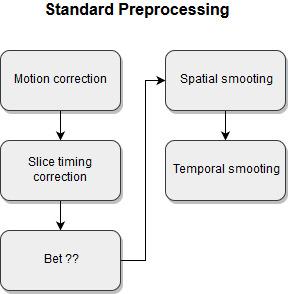
\includegraphics[width=.35\textwidth]{figures/bMethods/Standard_preprocessing} 
	\caption{Flowchart illustrating the steps in the standard preprocessing pipeline.}
	\label{fig:meth:std} 
\end{figure}

\subsection{Motion correction}

Correcting for motion artifacts when working with fMRI is nearly inevitable, since even the best subjects will not be able to hold still during acquisition. Even subtle movements as swallowing will be visible in the acquired image. \cite{Poldrack2011} To correct for these movement induced artifacts, a realignment of all volumes within a scan has been carried out using the FSL software program FMRIB's Motion Correction Linear Image Registration Tool (MCFLIRT). \cite{Jenkinson2002}
The tool was used to realign the series of images to a template image. The volume acquired halfway through the scan was used a reference image. This choice of template image is often justified by the middle volume being the closets to the average as well as the scanner at that time would have achieved maximum stability, as the magnetization would have reached steady state. \cite{Poldrack2011} A 6 degree of freedom transformation was used to realign the images, and can therefore only correct for bulk motion. \cite{Jenkinson2002}




\subsection{Slice timing correction}

When acquiring fMRI scans the slices in each volume are taken one by one. This can either be in an ascending, descending or interleaved order. Interleaved order is sequentially skipping every either odd or even slice and then afterwards acquiring the skipped slices. Ascending and descending is either from top to bottom or the opposite. Regardless of which order the slices were acquired, a misrepresentation of the hemodynamic response in each slice to the same hemodynamic response will be present due to the time difference in the slices. A representation of this effect can be seen in \figref{fig:meth:slice}. The difference in timing for each slice constitutes a problem when analyzing the data. The data is formed into statistical model, but since this model assumes that all slices are acquired at the same time point, the actual signal and the estimated in the statistical model creates a mismatch. \cite{Poldrack2011} \\

\begin{figure}[H] 
	{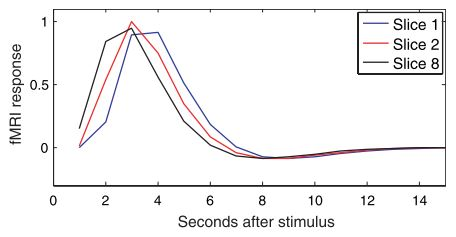
\includegraphics[width=.65\textwidth]{figures/aBackground/response}}  
	\caption{An illustration of the slice-wise acquisition effects the representation of the hemodynamic response. The response will seem to appear earlier in slice one compared to the others, as it is always the first acquired throughout the scan. \cite{Poldrack2011}}
	\label{fig:meth:slice}
\end{figure}

To account for the mismatch in the acquisition time of each slice, a correction has been implemented using FSL software \cite{FMRIB2018}. This is done by supplying the algorithm with acquisition order and the TR period. Hence, regular up and 2 second were inputed. The slice timing works by shifting the time series for the hemodynamic response curve for each slice in time to fit the middle of the TR period. This is achieved using Hanning windowed sinc interpolation. Choosing the middle slice as the reference, introduces the less interpolation, and is therefore seen as the most accurate method. \cite{Poldrack2011} Hence, the slice timing correction is carried out for each of the 193 volumes in a scan. 

%The standard algorithm for slice timing correction uses sinc interpolation between time points, which is accomplished by a Fourier transform of the signal at each voxel. The Fourier transform renders any signal as the sum of some collection of scaled and phase-shifted sine waves; once you have the signal in that form, you can simply shift all the sines on a given slice of the brain forward or backward by the appropriate amount to get the appropriate interpolation. There are a couple pitfalls to this technique, mainly around the beginning and end of your run, highlighted in Calhoun et. al below, but these have largely been accounted for in the currently available modules for slice timing correction in the major programs.
    

\subsection{Brain extraction}

This step is the brain extraction of the brain in the functional scan. The extraction of the functional brain is done in the same way as presented in \secref{BET}. 
\subsection{Spatial smoothing}

The next step in the standard preprocessing approach was to introduce spatial smoothing. Some of the image pixels will likely be contaminated with scattered noise presented higher pixel intensities. These can be removed by averaging the misrepresented pixel with its surrounding neighbors. Hence, this allows for the possibility of gaining a higher signal to noise ratio though with the consequence of a decrease in spatial resolution as the image gets blurred and smaller areas of activation gets smeared together. The operation can be justified by the closely neighboring voxel being correlated in effect to the hemodynamic response. Thereby some of the higher-frequency information removed by spatial smoothing. Furthermore spatial smoothing has the advantage that is reduces reduces the difference between subjects improving the between subject comparison. \cite{Poldrack2011} \\
The implementation of spatial smoothing on the data was done using the Smoothing over Univalue Segment Assimilating Nucleus (SUSAN) noise reduction filter in the FSL toolbox. The 3 dimensional spatial smoothing was carried out on each volume of the FMRI data set separately. Thereby reducing noise without reducing valid activation, which should be achieved using a mask size of 5 mm full width half maximum (FWHM), thus resulting in a trade off of smoothing bigger and smaller areas of activation. An advantage of the SUSAN algorithm is its ability to distinguish between tissue types as e.g. grey matter and white matter and thereby only including intensity value from neighboring voxels which consist of the same tissue type as the voxel being smoothened. Thereby all structures in the image should be preserved. \cite{Smith1997}  


\subsection{Temporal smoothing}

A characteristic noise which represents itself during fMRI data is the presence of a low-frequency drift. The drift is characterized as a slow increasing trend in the BOLD magnitude, when assessing the signal in the time domain. Doing a Fourier Transform, to analyze the signal in the power spectrum, would reveal low frequency contributers influencing the signal. As mentioned in \secref{ac}, the frequency of noise was 0 Hz to 0.015 Hz and the frequency band of activation is 0.01 Hz to 0.02 Hz. To dampen some of the low-frequency artifactual content a high pass filter with a cutoff frequency of 100 seconds (0.01 Hz) was implemented. \cite{FMRIB2018}. \\


 
 % The reason for this type of noise contamination has been heavily investigated, and conclusions state that the noise originates from MRI scanner instability. As this low-frequency drift will always be present, it is very crucial to consider the interval of which tasks or stimuli are performed to avoid the output being present in the noise range of $0$ to $0.015$ Hz. Therefore stimuli or tasks should be performed within intervals of $70$ s or less. \cite{Poldrack2011} \\ 
 
 
 
 
